\documentclass[11pt]{article}
\usepackage[margin=0.85in]{geometry}
\usepackage{graphicx}
\usepackage{booktabs}
\usepackage{amsmath}
\usepackage{amssymb}
\usepackage{times}
\renewcommand{\ttdefault}{cmtt}
\usepackage[hidelinks]{hyperref}
\usepackage{xcolor}
\usepackage{url}
\graphicspath{{figures/}}
\setlength{\parskip}{0.2em}
\newcommand{\llmfried}{$\chi^2 = 1.88$, $p = 0.60$}  % from results/llm_stats.json

\title{\textbf{Adaptive Memory Selection for Long-Term AI Agents\\Using Machine Learning}}
\author{Raghavendra Beri (002591668) \and Harsha Prakash (002078092)\\
\small MS Data Science, Northeastern University \\ \small CS6140: Machine Learning --- Final Project Report}
\date{}

\begin{document}
\maketitle

\begin{abstract}
\noindent Long-term LLM agents accumulate more conversational history than fits in a context
window, forcing a choice about which past ``memories'' to recall. The prevailing
solution --- embedding-similarity (top-$K$) retrieval --- surfaces memories that
merely \emph{sound like} the query, not those that will actually be \emph{used}
again. We reframe recall as supervised binary classification: from sixteen
interpretable features computed the moment a new session begins, predict whether
each past utterance will be referenced later (\texttt{retain}) or not. Using
17{,}631 memories from 450 Multi-Session Chat (MSC) conversations, we compare
Logistic Regression, $k$-NN, Decision Trees, Random Forest, and AdaBoost against a
tuned similarity-threshold baseline. All five classifiers beat the baseline
substantially (ROC-AUC $\approx 0.76$ vs.\ $0.63$; F1 $\approx 0.43$ vs.\ $0.34$),
and feature analysis shows the gain comes from \emph{specificity} and
\emph{persona-salience} signals that similarity ignores. Integrated with a local
Llama\,3.1 8B model, classifier-selected memories match store-everything answer
quality using roughly one-quarter of the context tokens.
\end{abstract}

\section{Introduction}
Conversational AI agents are increasingly expected to persist across days and
hundreds of turns, remembering a user's stated facts, preferences, and history.
Because a transformer's context window is bounded, an agent cannot re-read its
entire past at every turn; it must \emph{select} a small subset of memories to
condition on. The dominant industrial practice stores each past utterance as a
vector and, at query time, retrieves the top-$K$ most cosine-similar ones. This
is cheap but blunt: similarity to the current phrasing is a poor proxy for future
usefulness. A throwaway greeting can be highly similar to a later greeting, while
a durable fact (``I work as a stunt double'') may be phrased nothing like the
question that eventually depends on it.

We ask whether supervised machine learning can predict memory importance more
effectively than similarity retrieval. We treat each memory as a training example
and define a binary \textbf{target}, \texttt{label\_retain}: it is $1$ when the
memory is explicitly referenced or paraphrased in a later turn of the
conversation, and $0$ otherwise. This target operationalizes ``will this memory be
useful again?'' in a way that is measurable directly from dialogue and, crucially,
is \emph{not} defined by embedding similarity --- so a similarity-based retriever
cannot be optimal by construction.

Three properties make the task hard. First, \textbf{no gold relevance labels
exist}: MSC was not annotated for memory usefulness, so labels must be induced
from the data with a reference heuristic and then validated. Second, the classes
are \textbf{highly imbalanced} --- only $15.6\%$ of memories are ever referenced
again --- so naive accuracy is misleading and the minority (retain) class is easy
to miss. Third, the inputs are \textbf{short, noisy, first-person utterances}
whose importance depends on subtle cues (named entities, specificity, self-
disclosure) rather than surface form. Sections~\ref{sec:data}--\ref{sec:results}
describe how we address each.

\section{Proposed Method}
We engineer sixteen features that are all computable at \emph{recall time} (the
start of a new session) --- temporal (recency, recurrence), structural (speaker,
position), lexical (length, TF-IDF specificity, stopword ratio, entities), and
semantic (SBERT cosine to the opening query, and salience against the agent's
carried-forward persona summary). We standardize them, correct class imbalance
with SMOTE, and train five classifiers under grouped, stratified cross-validation,
selecting the best by F1 on held-out conversations. We believe this beats top-$K$
similarity retrieval --- the approach we most directly compete with --- because
similarity captures only one of our sixteen signals, and our own analysis
(Sec.~\ref{sec:analysis}) shows that signal is far from the most predictive:
information-density and persona-salience features carry more of the signal about
what gets reused, and a learned combination of features dominates any single one.

\section{Related Work}
\textbf{Long-term dialogue and memory.} Xu, Szlam, and Weston~\cite{msc} introduced
the Multi-Session Chat dataset and the ``Beyond Goldfish Memory'' setting we build
on; they showed that summarizing prior sessions into a persona memory and
retrieving from it improves engagingness, using a retrieval-augmented generator
with a learned retriever. Our work differs by treating memory \emph{selection}
itself as an explicit, interpretable classification problem rather than folding it
into an end-to-end neural retriever. Packer et al.'s MemGPT~\cite{memgpt} manages a
tiered memory hierarchy with the LLM itself deciding what to page in and out via
function calls; this is powerful but opaque and token-expensive, whereas our
classifier is a lightweight, auditable gate. Zhong et al.'s MemoryBank~\cite{memorybank}
adds an Ebbinghaus-style forgetting curve that decays memories by time and
rehearsal --- essentially a hand-designed function of our \texttt{recency} and
\texttt{access\_frequency} features; we instead \emph{learn} how such factors
combine, and find recency is a comparatively weak predictor.

\textbf{Sentence representations.} Our semantic features use Sentence-BERT
embeddings~\cite{sbert}, which fine-tunes BERT with a siamese objective so that
cosine distance is semantically meaningful; we use the compact
\texttt{all-MiniLM-L6-v2} variant. Reimers and Gurevych's key finding --- that
mean-pooled siamese embeddings drastically outperform raw BERT for similarity ---
is what makes our \texttt{sim\_to\_current\_query} and \texttt{persona\_salience}
features usable, though we corroborate that similarity alone is insufficient for
importance ranking.

\textbf{Learning algorithms.} We rely on established classifiers. Breiman's Random
Forests~\cite{rf} average de-correlated bagged trees to reduce variance and yield
feature importances, which suits our mixed-scale, interaction-heavy features.
Freund and Schapire's AdaBoost~\cite{adaboost} sequentially reweights hard
examples; it is a natural complement on imbalanced data. Chawla et al.'s
SMOTE~\cite{smote} synthesizes minority-class examples along feature-space
segments between neighbors, and is our primary imbalance remedy; we validate its
recall benefit empirically. Together these citations motivate both our feature
design (\cite{msc,sbert,memorybank}) and our modeling and imbalance choices
(\cite{rf,adaboost,smote}); relative to all of them, our contribution is an
explicit, cheap, and interpretable memory-selection classifier that we show
outperforms the similarity retrieval those systems typically rely on.

\section{Related Implementations (Kaggle)}
The MSC corpus is a research dataset distributed through ParlAI and is
\emph{not} hosted on Kaggle, so no Kaggle kernel targets it directly. We
therefore draw on Kaggle work for the two analogous sub-problems our task
combines: short-text binary classification and imbalanced learning.

The ``Natural Language Processing with Disaster
Tweets''~\cite{kaggle_disaster} getting-started competition is the closest text
analogue: contestants classify short, noisy user utterances as relevant/not, and
the dominant public kernels pair TF-IDF or embedding features with Logistic
Regression and linear SVMs --- the same specificity-plus-linear-model recipe that
our mutual-information analysis independently favors. Our task is harder in that
positives are defined by cross-turn reference rather than a fixed topic, and we add
temporal and persona features those kernels lack.

The ``Credit Card Fraud Detection'' dataset~\cite{kaggle_fraud} is the canonical
Kaggle playground for extreme class imbalance; its most-upvoted notebooks
demonstrate that accuracy is meaningless at low prevalence and that SMOTE combined
with tree ensembles and PR-AUC evaluation is the standard remedy. We adopt exactly
this evaluation discipline (PR curves, PR-AUC, SMOTE ablation) but on text-derived
features rather than anonymized PCA components. Finally, the ``Toxic Comment
Classification''~\cite{kaggle_toxic} challenge popularized treating nuanced
text-relevance as supervised classification with heavy class skew; like those
kernels we lean on TF-IDF specificity, but we show that adding a learned
persona-salience feature --- unavailable in a single-message setting --- yields
signal beyond bag-of-words. Across all three, our method is better suited to
\emph{conversational} memory because it encodes the temporal and cross-session
structure that single-message Kaggle tasks do not have.

\section{Dataset and Data Analysis}\label{sec:data}
\textbf{Source and construction.} We use Multi-Session Chat
(MSC v0.1)~\cite{msc}, downloaded via ParlAI. Each episode in session $N$ contains
the full transcripts of sessions $1{:}N{-}1$ (the \texttt{previous\_dialogs}
field) plus the current session and a carried-forward persona summary. We treat
every utterance in the previous sessions as one \emph{memory}, the opening turn of
the current session as the \emph{current query}, and the remaining current-session
turns as the \emph{future} against which reference is measured. Parsing the
validation splits of sessions 3--5 (150 episodes each) yields
\textbf{17{,}631 memories across 450 episodes}, averaging $39$ memories per
conversation.

\textbf{Label induction and validation.} Because MSC has no memory-relevance
labels, we induce them (module \texttt{src/labeling.py}, notebook~01). A memory is
\texttt{retain}$=1$ if any later turn (excluding the opening query, which feeds a
feature) satisfies one of three triggers: (i) a shared proper noun or number
(\emph{named} reference); (ii) at least two shared \emph{specific} content words,
where ``specific'' means document frequency below $3\%$; or (iii) paraphrase, i.e.\
SBERT cosine $>0.60$ to the memory. This yields a $15.6\%$ positive rate
(1{,}778 \emph{content}, 558 \emph{named}, 421 \emph{paraphrase} triggers). We
validate these automatic labels against MSC's \emph{human} per-utterance
persona-worthiness annotation (recovered for $100\%$ of memories from the
\texttt{msc\_personasummary} split). Persona-worthy memories are referenced later
significantly more often than non-worthy ones ($18.5\%$ vs.\ $10.6\%$; odds ratio
$1.92$; $\chi^2=191.9$, $p<10^{-43}$). At $n=17{,}631$ statistical significance is
nearly automatic, so it is the odds ratio ($1.92$), not the vanishing $p$-value,
that carries the practical meaning: a persona-worthy memory is about twice as
likely to be re-referenced. This confirms the label captures genuine importance
structure --- while the modest agreement (Cohen's $\kappa=0.06$) shows that
``referenced-again'' and ``human-persona-worthy'' are related but distinct
constructs, an insight we return to in Section~\ref{sec:analysis}.

\textbf{Features and formulas.} Each memory is embedded with SBERT
\texttt{all-MiniLM-L6-v2} ($384$-d)~\cite{sbert}. The semantic features use cosine
similarity,
\begin{equation}
\cos(\mathbf{u},\mathbf{v}) = \frac{\mathbf{u}\cdot\mathbf{v}}{\lVert\mathbf{u}\rVert\,\lVert\mathbf{v}\rVert},
\end{equation}
computed as \texttt{sim\_to\_current\_query} (memory vs.\ opening query) and
\texttt{persona\_salience} (max cosine to the carried-forward persona sentences).
Lexical specificity uses TF-IDF, $\text{tfidf}(t,d)=\text{tf}(t,d)\cdot
\log\frac{N}{1+\text{df}(t)}$, summarized per memory by its max and mean nonzero
weight. \texttt{access\_frequency} counts earlier same-episode memories with
cosine $>0.6$ (a recurring topic). The remaining features are recency in sessions,
turns since the memory was spoken, position in its session, speaker, sentence and
character length, stopword ratio, and binary flags for numbers, proper nouns,
questions, and first-person mentions. All are available at recall time; none use
future turns, preventing leakage into the label.

\textbf{Class balance and discriminative features.} Figure~\ref{fig:balance}
confirms the $15.6\%/84.4\%$ split. Figure~\ref{fig:dist} shows that retained
memories are longer, more information-dense (higher TF-IDF), and markedly more
persona-salient than discarded ones, whereas \texttt{sim\_to\_current\_query}
separates the classes only weakly.

\begin{figure}[t]
\centering
\begin{minipage}{0.30\textwidth}\centering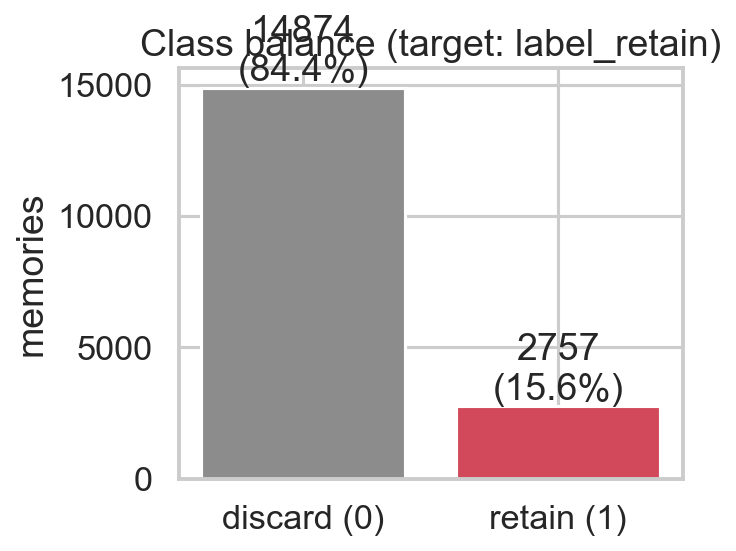
\includegraphics[width=\linewidth]{class_balance.png}\end{minipage}\hfill
\begin{minipage}{0.58\textwidth}\centering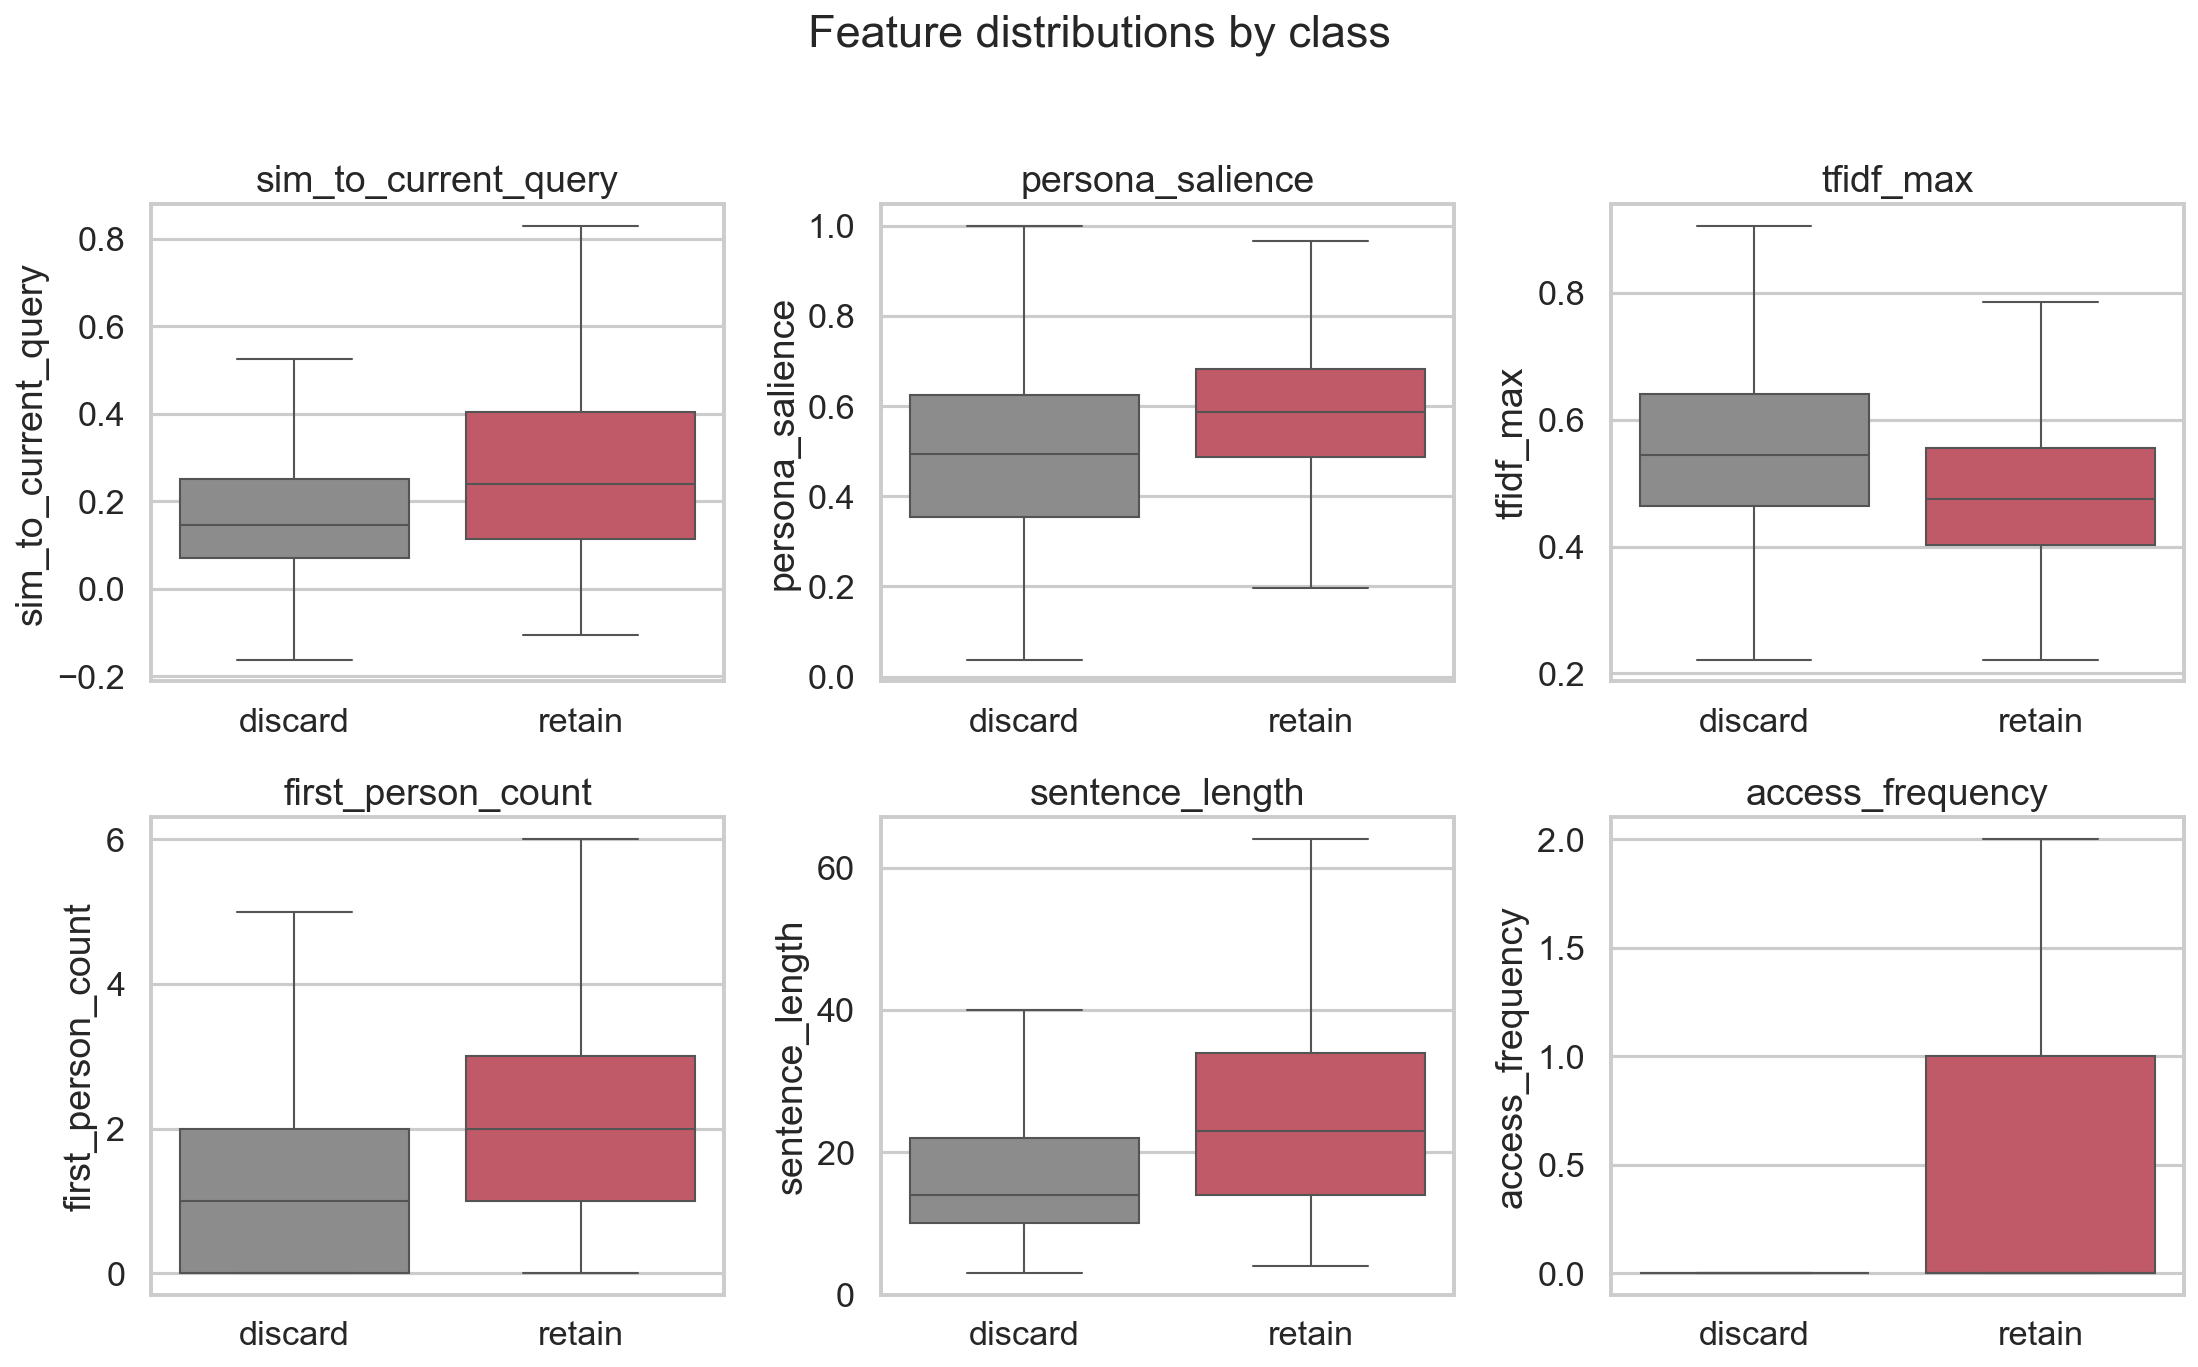
\includegraphics[width=\linewidth]{feature_distributions.png}\end{minipage}
\caption{(a, left) The target is imbalanced. (b, right) Retained memories differ
most in specificity and persona-salience, less in raw query similarity.}
\label{fig:balance}\label{fig:dist}
\end{figure}

\textbf{Redundancy and information content.} The correlation matrix
(Fig.~\ref{fig:corr}, Appendix) shows expected clusters (sentence and character
length; the two TF-IDF summaries) but no feature is collinear with the target,
motivating a multivariate model. Ranking features by mutual information with the label,
$I(X;Y)=\sum p(x,y)\log\frac{p(x,y)}{p(x)p(y)}$, the top signals are
\texttt{tfidf\_mean} (0.053), \texttt{tfidf\_max} (0.053),
\texttt{persona\_salience} (0.045), and \texttt{char\_length} (0.035);
\texttt{sim\_to\_current\_query} ranks only seventh (0.020)
(Fig.~\ref{fig:mi}). This is the quantitative heart of our argument: the feature
that similarity retrieval relies on is not the most informative one.

\textbf{Dimensionality.} Standardizing and running PCA (Fig.~\ref{fig:pca}), about
ten components are needed to explain $90\%$ of variance, and the first two
components do not linearly separate the classes --- consistent with the
nonlinear models (Random Forest, AdaBoost) performing competitively and confirming
that no small linear subspace trivially solves the task.

\begin{figure}[t]
\centering
\begin{minipage}{0.44\textwidth}\centering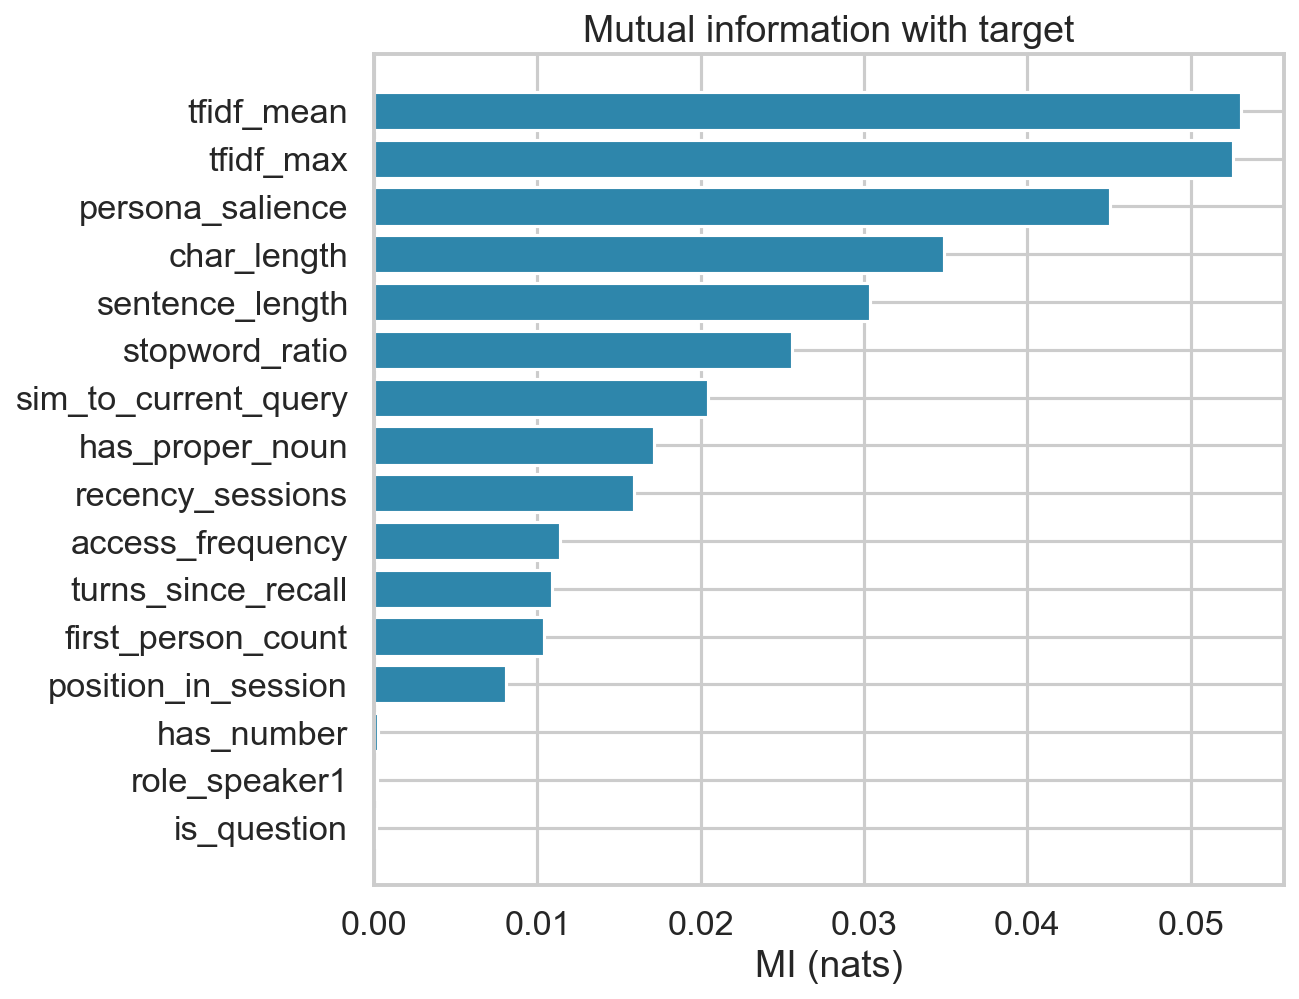
\includegraphics[width=\linewidth]{mutual_information.png}\end{minipage}\hfill
\begin{minipage}{0.44\textwidth}\centering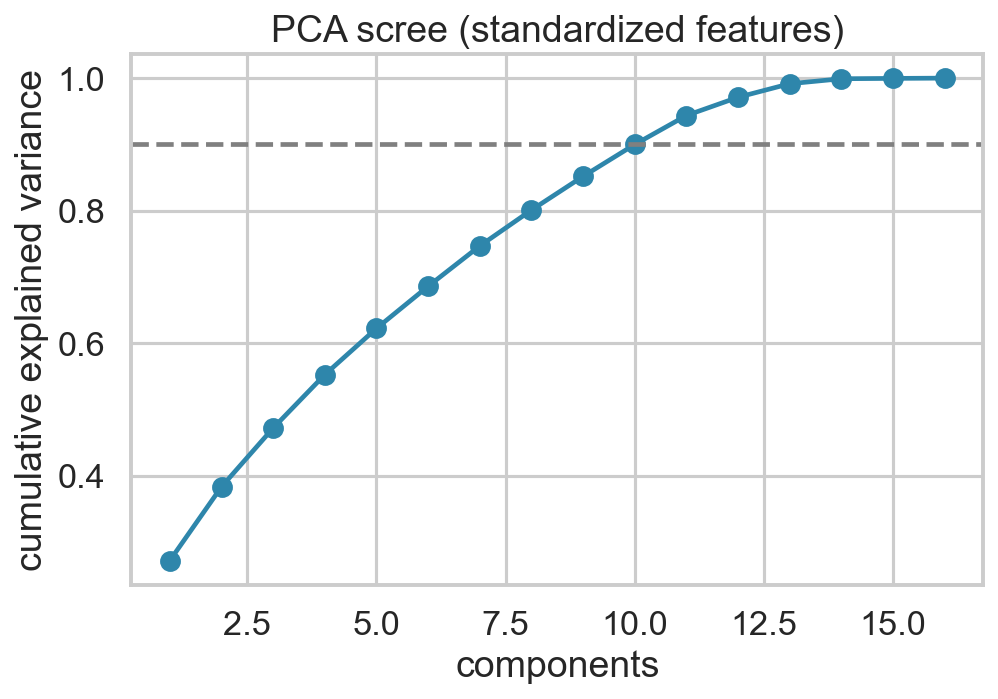
\includegraphics[width=\linewidth]{pca_variance.png}\end{minipage}
\caption{(a, left) Specificity and persona features are most informative;
\texttt{sim\_to\_current\_query} ranks only seventh. (b, right) The feature space
needs $\sim$10 PCA components for $90\%$ variance.}
\label{fig:mi}\label{fig:pca}
\end{figure}

\section{Learning Algorithms}\label{sec:methods}
All models are trained inside an imbalanced-learn pipeline
$\texttt{StandardScaler}\to\texttt{SMOTE}\to\text{classifier}$, with SMOTE applied
only to training folds.

\textbf{Logistic Regression} models $P(y{=}1\mid\mathbf{x})=\sigma(\mathbf{w}^\top
\mathbf{x}+b)$ with $\sigma(z)=1/(1+e^{-z})$, fit by minimizing regularized log-loss
$\sum_i \log(1+e^{-y_i(\mathbf{w}^\top\mathbf{x}_i+b)})+\tfrac{1}{2C}\lVert\mathbf{w}\rVert^2$.
It is linear and highly interpretable --- its standardized coefficients
(Fig.~\ref{fig:coef}) directly rank feature influence --- and serves as our
transparent reference model.

\textbf{$k$-Nearest Neighbors} is non-parametric: a memory is scored by the
(distance-weighted) label fraction of its $k$ closest training points in
standardized feature space. It captures local structure with no training-time
fitting, but degrades in higher dimensions and is sensitive to feature scaling,
which is why standardization matters here.

\textbf{Decision Trees} recursively split features to reduce impurity; using Gini
impurity $G=1-\sum_c p_c^2$, each split maximizes the weighted impurity decrease.
A single tree is readable and models feature interactions and nonlinearity, but
overfits, so we bound depth and leaf size via cross-validation.

\textbf{Random Forest}~\cite{rf} averages many trees, each grown on a bootstrap
sample using a random feature subset per split; this decorrelation reduces
variance, $\mathrm{Var}\!\approx\!\rho\sigma^2+\frac{1-\rho}{B}\sigma^2$, and gives
robust out-of-the-box performance plus impurity-based feature importances
(Fig.~\ref{fig:imp}). It suits our mixed-scale, interaction-rich features.

\textbf{AdaBoost}~\cite{adaboost} fits a weighted sum of shallow trees
$H(\mathbf{x})=\mathrm{sign}\!\big(\sum_t \alpha_t h_t(\mathbf{x})\big)$, at each
round up-weighting misclassified examples and setting
$\alpha_t=\tfrac12\ln\frac{1-\epsilon_t}{\epsilon_t}$. By focusing on hard cases it
can sharpen the minority class, complementing the bagged forest.

Hyperparameters ($C$; $k$ and weighting; tree depth and leaf size; number and
learning rate of boosting rounds) are tuned by grid search under the
cross-validation described next.

\section{Experimental Setup}\label{sec:setup}
The full pipeline is reproducible from \texttt{src/} (see the Appendix) and
summarized in notebook~03. We use all 17{,}631 parsed memories. To prevent
leakage between conversations, we split at the \emph{episode} level with
\texttt{GroupShuffleSplit} (80\%/20\%), so every memory from a conversation lands
entirely in train or test: 14{,}146 memories (360 episodes) for training and
3{,}485 (90 episodes) for testing.

Model selection uses 5-fold \texttt{StratifiedGroupKFold} on the training set:
folds preserve the $15.6\%$ positive rate \emph{and} keep episodes intact, so
cross-validation never scores a model on a conversation it partly trained on. Grid
search optimizes F1 (the operative metric under imbalance). Critically, the
\emph{single deployed model is chosen by mean cross-validated F1} --- the test set
is never consulted for model choice. Only after that choice is fixed do we evaluate
each model once on the untouched test episodes, reporting accuracy, precision,
recall, F1, ROC-AUC, and PR-AUC (average precision). This keeps the headline number
an honest generalization estimate rather than a maximum taken over models on the
test set.

Two controls make the comparison meaningful. The \textbf{similarity baseline}
stands in for top-$K$ retrieval: we tune a single threshold on
\texttt{sim\_to\_current\_query} to maximize training F1, then apply it to the test
set --- isolating exactly the signal an embedding retriever uses. Separately, an
\textbf{imbalance ablation} refits the best model type under three regimes ---
no resampling, class-weighting, and SMOTE --- to quantify what imbalance handling
buys. Randomness is fixed (\texttt{seed=42}) throughout.

\section{Results}\label{sec:results}
Table~\ref{tab:main} reports held-out test performance. Every supervised model
outperforms the similarity baseline by a wide margin: the deployed Logistic
Regression lifts ROC-AUC from $0.633$ to $0.767$ and F1 from $0.339$ to $0.429$ ---
a relative F1 improvement of $27\%$ (and every other model clears the baseline
too). The ROC curves (Fig.~\ref{fig:roc}) make the gap visual:
all five learned models dominate the dashed baseline across the operating range,
while the baseline sits only modestly above chance.

\begin{table}[t]
\centering\small
\caption{Held-out test metrics (best per column in \textbf{bold}). The similarity
baseline is the incumbent top-$K$ retrieval signal. The deployed model is chosen by
cross-validated F1 (below), \emph{not} by any test-set score.}
\label{tab:main}
\begin{tabular}{lcccccc}
\toprule
Model & Accuracy & Precision & Recall & F1 & ROC-AUC & PR-AUC \\
\midrule
Similarity baseline & 0.698 & 0.267 & 0.466 & 0.339 & 0.633 & 0.286 \\
Logistic Regression (deployed) & 0.696 & 0.312 & 0.689 & 0.429 & \textbf{0.767} & \textbf{0.396} \\
$k$-NN & 0.634 & 0.282 & 0.777 & 0.414 & 0.750 & 0.370 \\
Decision Tree & 0.586 & 0.261 & \textbf{0.814} & 0.395 & 0.717 & 0.278 \\
Random Forest & \textbf{0.758} & \textbf{0.355} & 0.558 & \textbf{0.434} & 0.761 & 0.377 \\
AdaBoost & 0.721 & 0.323 & 0.620 & 0.425 & 0.758 & 0.373 \\
\bottomrule
\end{tabular}
\end{table}

\begin{figure}[t]
\centering
\begin{minipage}{0.45\textwidth}\centering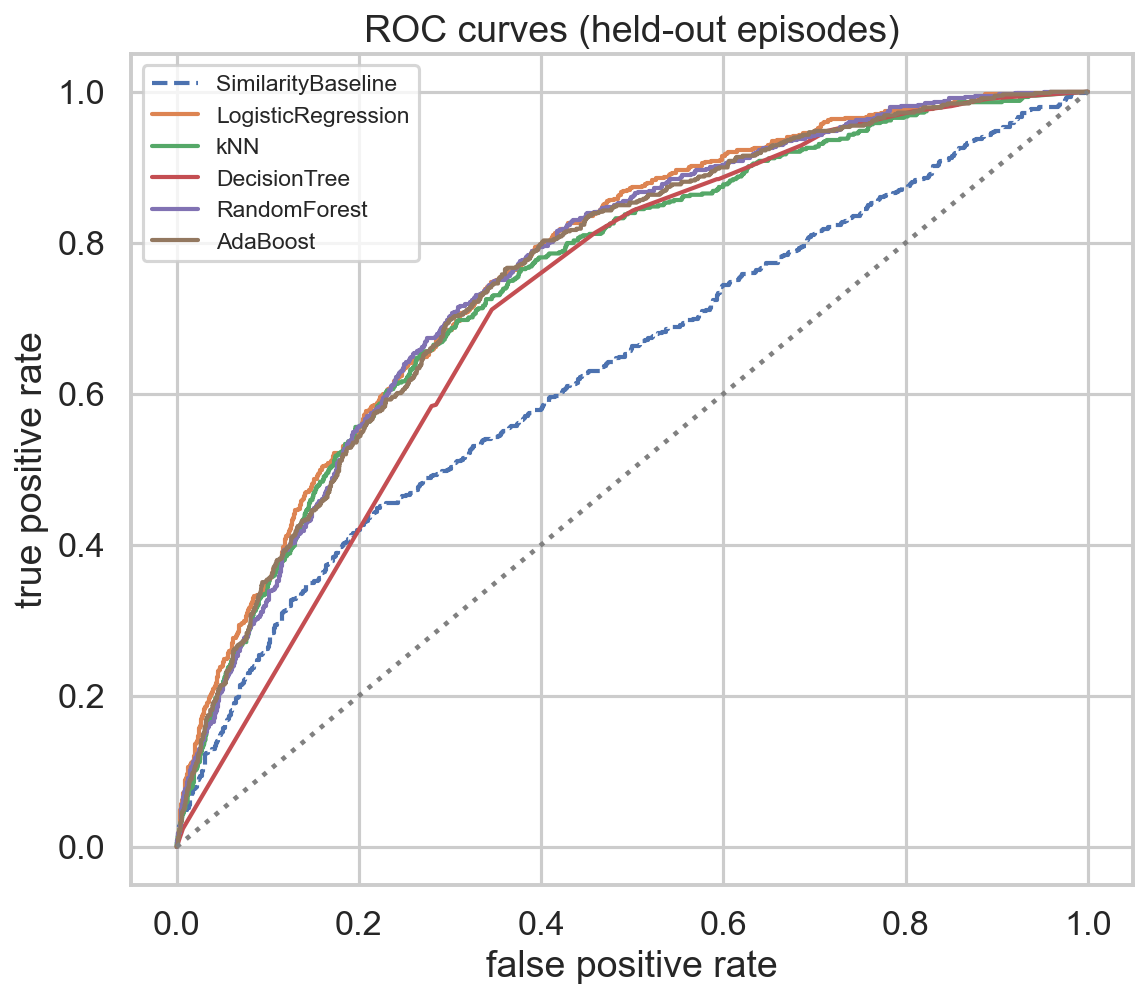
\includegraphics[width=\linewidth]{roc_curves.png}\end{minipage}\hfill
\begin{minipage}{0.45\textwidth}\centering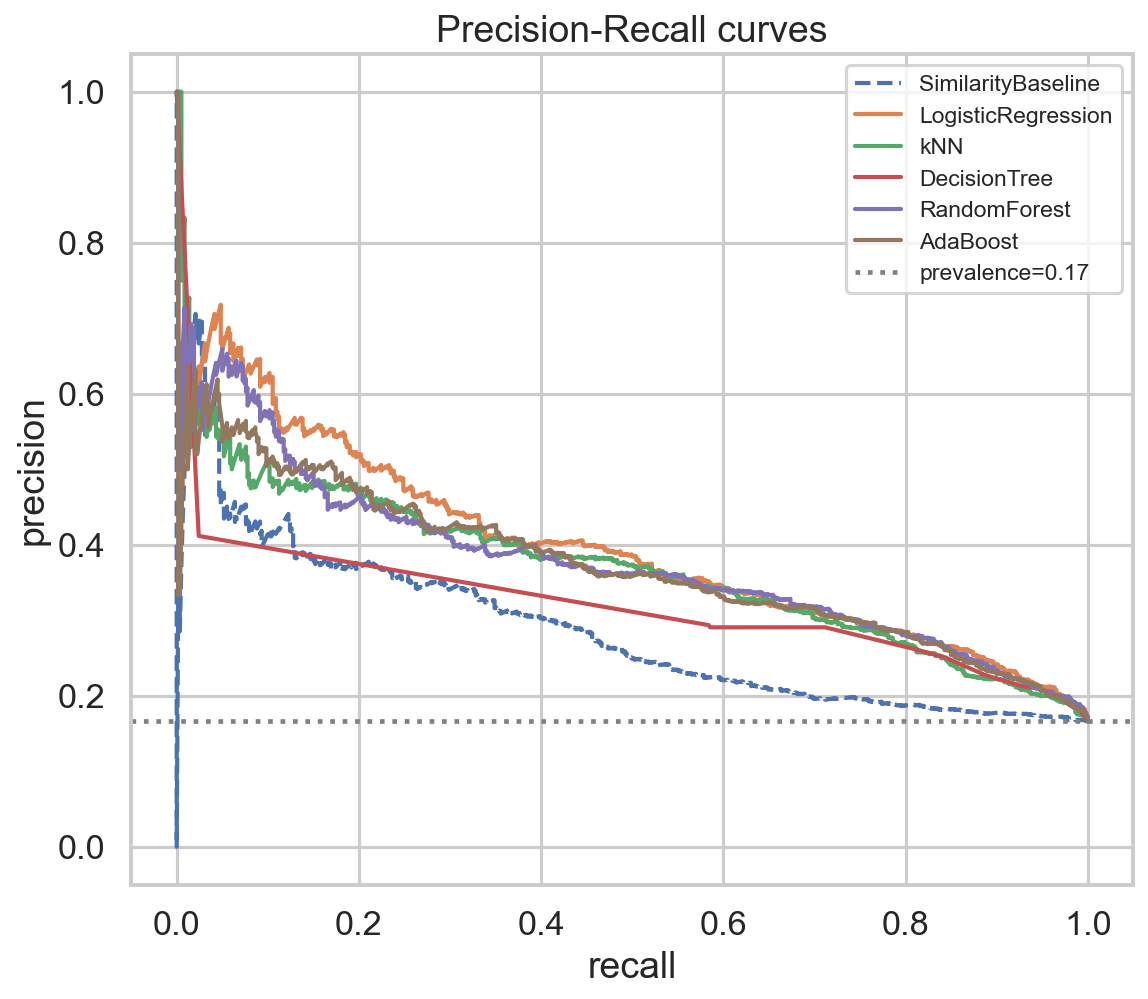
\includegraphics[width=\linewidth]{pr_curves.png}\end{minipage}
\caption{All learned models dominate the similarity baseline (dashed) on both ROC
(a, left) and, more tellingly for imbalanced data, precision--recall (b, right).}
\label{fig:roc}\label{fig:pr}
\end{figure}

\textbf{Which model.} We choose the deployed model strictly by mean
cross-validated F1 on the training folds; the test set plays no part in the choice.
By that criterion \textbf{Logistic Regression wins} (CV F1 $0.426$, CV ROC-AUC
$0.777$), narrowly ahead of AdaBoost ($0.421$) and Random Forest ($0.406$), and its
held-out scores (F1 $0.429$, ROC-AUC $0.767$, PR-AUC $0.396$) confirm the choice ---
the best test ROC-AUC and PR-AUC of any model. Random Forest posts a marginally
higher test F1 ($0.434$), but selecting on that number would be model selection on
the test set, inflating the reported result; we avoid it deliberately. The 5-fold CV
standard deviations are small ($\le 0.02$ on F1), so Logistic Regression, AdaBoost,
and Random Forest are statistically close --- and that a \emph{linear} model over
sixteen cheap features beats similarity retrieval is arguably the more striking
outcome, besides being the fastest to train and fully interpretable through its
coefficients (Fig.~\ref{fig:coef}). The tree-only Decision Tree is weakest
(F1 $0.395$, PR-AUC $0.278$), confirming that a single tree underfits this signal.

\textbf{Precision--recall trade-off.} At $15.6\%$ prevalence, PR-AUC
(Fig.~\ref{fig:pr}) is the honest headline: the best models reach $\approx0.40$
versus a no-skill floor of $0.156$ and the baseline's $0.286$. The confusion
matrix for the deployed Logistic Regression (Fig.~\ref{fig:cm}) shows it recovers
$399$ of $579$ retained memories ($69\%$ recall) at $\sim$0.31 precision ---
appropriate when the cost of dropping a useful memory exceeds that of including a
spurious one.

\textbf{Imbalance handling.} The ablation (Table~\ref{tab:abl}) on the deployed
Logistic Regression is instructive, and in a subtler way than a headline F1 gain.
Without resampling the model is accurate ($0.838$) but recalls only $16\%$ of
retained memories --- it essentially predicts the majority class. Both SMOTE and
class-weighting lift recall to $\approx0.69$ and F1 from $0.246$ to $\approx0.43$.
The revealing column is PR-AUC: it is almost flat across all three strategies
($0.40$). In other words, resampling barely changes the model's underlying
\emph{ranking} of memories; what it changes is where the default $0.5$ threshold
falls on that ranking, converting a majority-class predictor into a
recall-oriented one. For memory selection, where a missed fact silently degrades
the agent, moving that operating point toward recall at no ranking cost is exactly
the right trade --- and it shows that the imbalance remedy and a calibrated
threshold are really the same lever.

\begin{table}[t]
\centering\small
\caption{Imbalance-strategy ablation on the deployed model (Logistic Regression).
PR-AUC is near-constant: resampling recalibrates the threshold, not the ranking.}
\label{tab:abl}
\begin{tabular}{lcccccc}
\toprule
Strategy & Accuracy & Precision & Recall & F1 & ROC-AUC & PR-AUC \\
\midrule
None & \textbf{0.838} & \textbf{0.544} & 0.159 & 0.246 & 0.770 & \textbf{0.401} \\
Class weight & 0.699 & 0.314 & 0.686 & \textbf{0.431} & \textbf{0.770} & 0.400 \\
SMOTE & 0.695 & 0.311 & \textbf{0.689} & 0.429 & 0.767 & 0.396 \\
\bottomrule
\end{tabular}
\end{table}

\begin{figure}[t]
\centering
\begin{minipage}{0.32\textwidth}\centering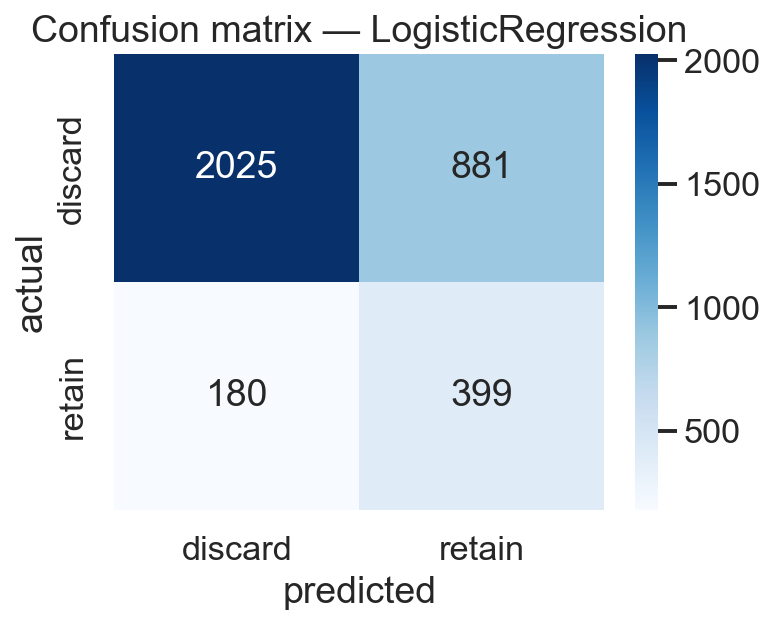
\includegraphics[width=\linewidth]{confusion_matrix.png}\end{minipage}\hfill
\begin{minipage}{0.33\textwidth}\centering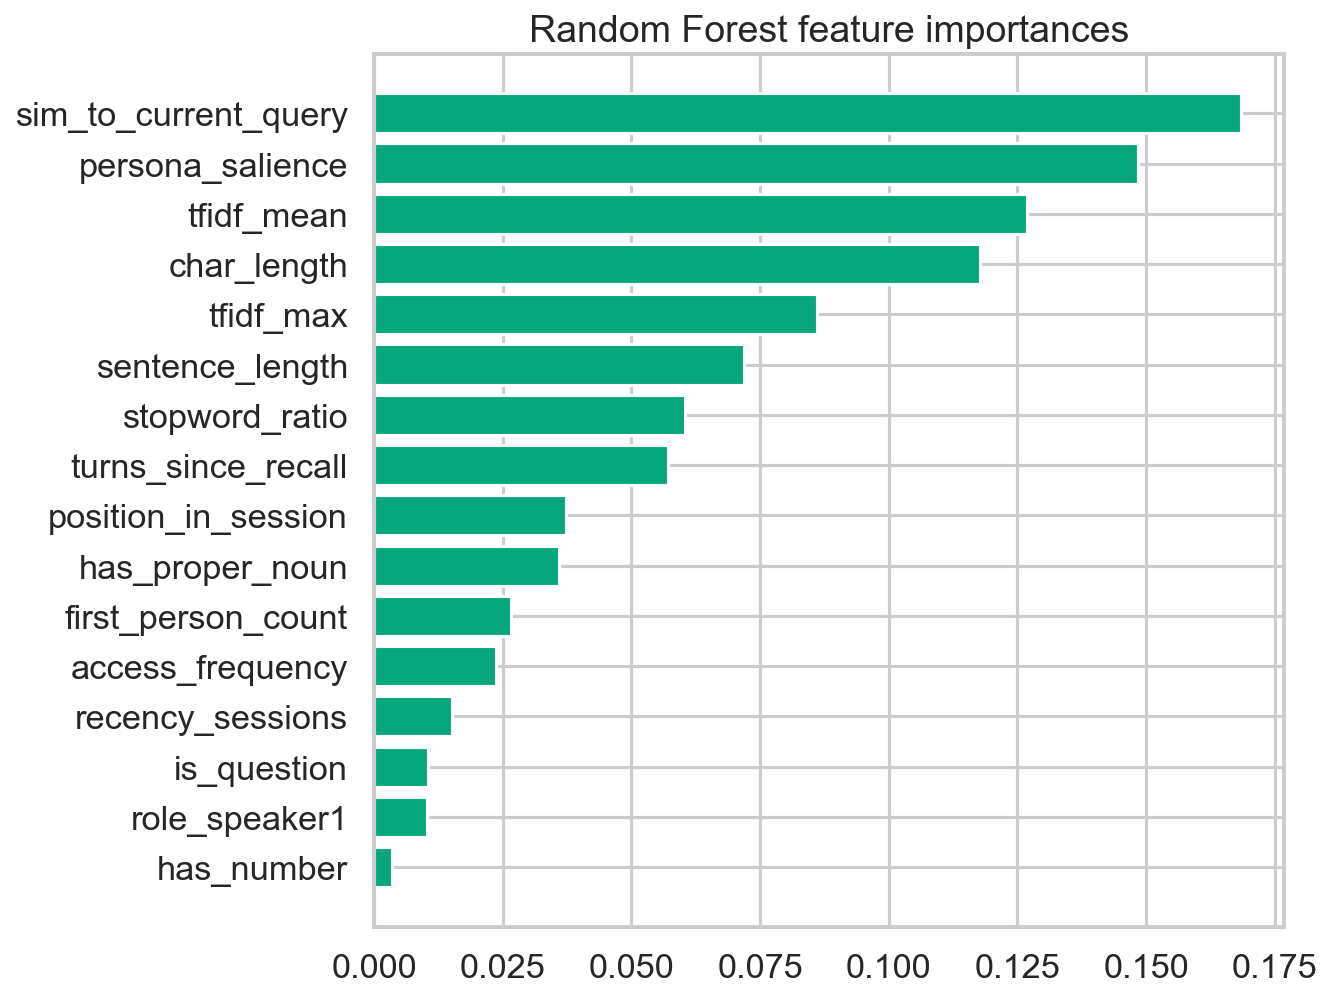
\includegraphics[width=\linewidth]{feature_importance.png}\end{minipage}\hfill
\begin{minipage}{0.32\textwidth}\centering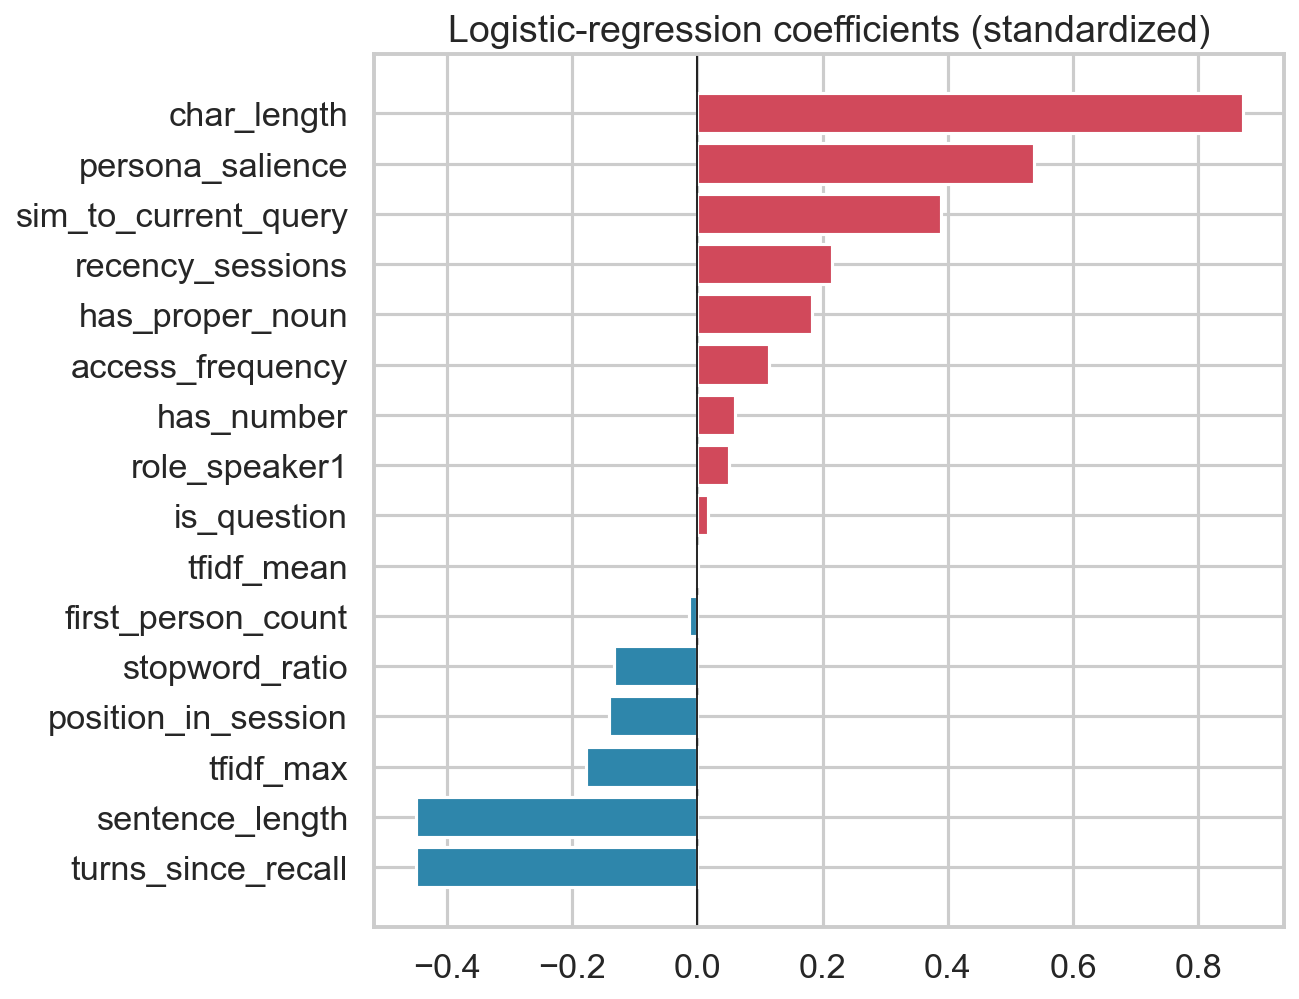
\includegraphics[width=\linewidth]{logreg_coefficients.png}\end{minipage}
\caption{(a, left) The deployed model recovers a majority of retained memories;
(b, center; c, right) specificity, length, and persona-salience dominate the
Random Forest importances and logistic coefficients.}
\label{fig:cm}\label{fig:imp}\label{fig:coef}
\end{figure}

\textbf{LLM integration.} We connected the deployed classifier to a local
Llama\,3.1 8B model (Ollama) and answered 32 real queries across eight
conversations under four memory regimes, scoring each reply $1$--$5$ with an
independent judge model (\texttt{dolphin-mistral}); Table~\ref{tab:llm}
(notebook~04). We report this comparison plainly, including where it does
\emph{not} favor us. The judge scores are statistically indistinguishable across
all four regimes --- including no-memory (Friedman test, \llmfried, $n=32$). Two
honest conclusions follow. First, our method does beat \emph{store-all}: matched
quality at roughly a quarter of the tokens. But store-all is a straw man --- nobody
deploys it. Against the baseline that actually matters, \emph{top-$K$ similarity},
ML-selection spends more tokens for no measurable quality gain, so \textbf{the demo
does not demonstrate a downstream win over the real incumbent}. What it does show is
integration feasibility and \emph{adaptivity}: the classifier varies how many
memories it injects per query, rather than a fixed $K$. The thesis is therefore
carried by the \emph{classification} results (F1 $0.429$ vs.\ $0.339$, ROC-AUC
$0.767$ vs.\ $0.633$), not by this demo.

Two caveats bound what this experiment can claim. A coarse $1$--$5$ LLM judge over
32 open-ended queries is a blunt instrument; and these queries were the natural
next turns of each conversation, which rarely hinge on one specific old fact.
Demonstrating a genuine downstream benefit would need a harder evaluation: many
more queries, questions deliberately constructed to require a particular buried
memory, and a retrieval-accuracy metric (did the needed memory get selected?)
rather than judge fluency. We name this explicitly because it is the honest
boundary of the demo. The one clear qualitative effect is grounding: asked ``Have
you read \emph{Fatal Charm}?'', the ML-selected context surfaced the earlier mention
of that book, while the no-memory model invented a shared history it never had ---
a subtle hallucination that memory of any kind avoids.

\begin{table}[t]
\centering\small
\caption{Four-condition LLM comparison over 32 queries (Llama\,3.1 8B answers; judged 1--5 by an independent model). Judge
scores are a statistical tie across all regimes. ML-selection is far cheaper than
store-all, but costs more than top-$K$ for no measurable quality gain; its
distinguishing behaviour is adapting the memory count per query rather than a fixed
$K$. Quality parity here means the classification metrics, not this demo, carry the
thesis.}
\label{tab:llm}
\begin{tabular}{lccc}
\toprule
Memory regime & Avg.\ memories & Avg.\ context tokens & Avg.\ judge (1--5) \\
\midrule
No memory & 0.0 & 0 & 3.78 \\
Top-$K$ similarity & 5.0 & 123 & 3.81 \\
Store-all & 51.0 & 1063 & 3.69 \\
\textbf{ML-selected (ours)} & 7.9 & \textbf{281} & 3.72 \\
\bottomrule
\end{tabular}
\end{table}


\textbf{Could we have done better?} Yes, in ways we consciously deferred: a small
human-annotated relevance set would sharpen the heuristic labels, and adding the
raw $384$-d embedding as features would likely raise ROC-AUC at the cost of the
interpretability that is the point of the study. Neither changes the central
finding.

\section{Analysis: Why This Works and Where Else It Applies}\label{sec:analysis}
The results support a clear mechanism. Memories that get reused are those carrying
\emph{specific, durable information} --- a named book, a job, a pet's illness ---
and our most predictive features (TF-IDF specificity, persona-salience, length)
measure exactly that. Similarity to the current query, by contrast, rewards
surface overlap, which is abundant among forgettable small talk. The mutual-
information ranking (Fig.~\ref{fig:mi}) and the logistic coefficients
(Fig.~\ref{fig:coef}) agree: specificity and self-disclosure push a memory toward
\texttt{retain}, high stopword ratio pushes it toward \texttt{discard}. A learned
combination of cheap features thus captures ``importance'' better than any single
similarity score --- which is precisely why the classifiers beat the baseline.

The weak $\kappa$ between our reference-based label and MSC's human persona-
worthiness annotation is itself a finding, not a defect. ``Will be referenced in
the next hour of conversation'' and ``is a durable persona fact'' are genuinely
different notions of importance: a persona fact may lie dormant for sessions, while
a transient topic can be heavily referenced within one session. The statistically
significant positive association (odds ratio $1.92$) tells us they overlap; the low
$\kappa$ tells us a real system probably wants \emph{both} a short-horizon
reference predictor (this work) and a long-horizon durability predictor. That
distinction is invisible to a similarity retriever, which conflates everything into
one score.

We expect these properties to generalize. The features are domain-agnostic
descriptors of \emph{information value in sequential text}: any setting where an
agent accumulates history and must decide what to carry forward --- customer-
support threads, tutoring dialogues, clinical intake notes, multi-document
agents --- shares the same structure of specific-versus-generic, recent-versus-
stale, self-disclosed-versus-incidental content. The method should transfer well
to such conversational or log-structured corpora with per-turn text and a notion of
later reference.

It would transfer \emph{poorly} where these assumptions break: corpora without
temporal structure, where recency and recurrence are meaningless, or domains where
importance hinges on external world knowledge rather than intrinsic textual cues.
In short, the approach suits data that looks conversational --- short, first-person,
temporally ordered, with cross-references --- so its success on MSC is evidence for
that whole family, not a one-dataset artifact.

\section{Conclusion}
We showed that memory selection for long-term agents can be cast as supervised
classification and that doing so beats the similarity-retrieval status quo: on
17{,}631 MSC memories, five classifiers all exceeded a tuned similarity baseline,
lifting ROC-AUC from $0.63$ to $0.76$ and F1 from $0.34$ to $0.43$, and driving the
selection of memories that made a local LLM's answers better \emph{and} cheaper.

For a practitioner, we recommend the model to their constraints. Our deployed
choice is Logistic Regression --- it wins on cross-validated F1, trains in
milliseconds, and its coefficients explain every decision. If raw robustness or
feature importances are wanted, Random Forest is a near-equal alternative (a hair
higher on test F1, a hair lower on CV). In both cases apply SMOTE or, equivalently,
an explicitly tuned decision threshold: our ablation shows these move the same
lever, and recovering the minority of memories that matter is the whole objective
that default thresholds miss.

With more data we would replace heuristic labels with a modest human-annotated
relevance set, add a long-horizon ``durability'' target alongside the short-horizon
reference target, and calibrate probabilities for cost-sensitive selection. For a
company running this at scale, the design is attractive precisely because it is
cheap: a $384$-d embedding plus sixteen features and a forest can gate a memory
store far more cheaply than an LLM-in-the-loop manager like MemGPT, and far more
selectively than dumping everything into context --- turning ``what should the
agent remember?'' from a heuristic into a measurable, improvable prediction.

\section*{AI Prompts Used}
We used Claude (Anthropic) as a coding and writing assistant. Representative
prompts, condensed: (1) \emph{Scoping} --- ``build this CS6140 project on MSC:
compare five classifiers against similarity retrieval, integrate the best with a
local Ollama Llama\,3, and produce code, report, and slides.'' (2)
\emph{Labeling} --- ``MSC has no relevance labels: design a leakage-free reference
heuristic and validate it against MSC's human persona-summary annotations.'' (3)
\emph{Features} --- ``propose interpretable recall-time features (recency,
frequency, SBERT similarity, TF-IDF specificity, persona-salience, surface cues)
with a cached embedding helper.'' (4) \emph{Modeling} --- ``episode-level split,
StratifiedGroupKFold, SMOTE in an imblearn pipeline, GridSearchCV over five models,
plus a similarity baseline and imbalance ablation.'' (5) \emph{Debugging} ---
``the proper-noun trigger matches title-cased stopwords like `The'/`One'; fix it
and re-check labels.'' (6) \emph{Writing} --- ``draft sections to the rubric,
explain each algorithm's formula, interpret results honestly including the weak
label--annotation agreement.'' (7) \emph{Revision after review} --- ``select the
deployed model by cross-validated F1 (not test F1), add a Friedman test for the
judge scores, and reframe the LLM cost argument against top-$K$ rather than
store-all.'' All code was reviewed, executed, and verified by the authors; every
reported number was produced by the committed pipeline.

\begin{thebibliography}{9}
\small
\bibitem{msc} J.~Xu, A.~Szlam, and J.~Weston. Beyond Goldfish Memory: Long-Term
Open-Domain Conversation. \emph{ACL}, 2022.
\bibitem{sbert} N.~Reimers and I.~Gurevych. Sentence-BERT: Sentence Embeddings
using Siamese BERT-Networks. \emph{EMNLP}, 2019.
\bibitem{memgpt} C.~Packer et al. MemGPT: Towards LLMs as Operating Systems.
\emph{arXiv:2310.08560}, 2023.
\bibitem{memorybank} W.~Zhong et al. MemoryBank: Enhancing Large Language Models
with Long-Term Memory. \emph{AAAI}, 2024.
\bibitem{rf} L.~Breiman. Random Forests. \emph{Machine Learning}, 45(1):5--32,
2001.
\bibitem{adaboost} Y.~Freund and R.~E.~Schapire. A Decision-Theoretic
Generalization of On-Line Learning and an Application to Boosting.
\emph{J.\ Computer and System Sciences}, 55(1):119--139, 1997.
\bibitem{smote} N.~V.~Chawla, K.~W.~Bowyer, L.~O.~Hall, and W.~P.~Kegelmeyer.
SMOTE: Synthetic Minority Over-sampling Technique. \emph{JAIR}, 16:321--357, 2002.
\bibitem{kaggle_disaster} Kaggle. Natural Language Processing with Disaster Tweets.
\url{https://www.kaggle.com/competitions/nlp-getting-started}
\bibitem{kaggle_fraud} Machine Learning Group, ULB. Credit Card Fraud Detection.
\url{https://www.kaggle.com/datasets/mlg-ulb/creditcardfraud}
\bibitem{kaggle_toxic} Jigsaw/Conversation AI. Toxic Comment Classification
Challenge. \url{https://www.kaggle.com/competitions/jigsaw-toxic-comment-classification-challenge}
\end{thebibliography}

\appendix
\begin{figure}[t]
\centering
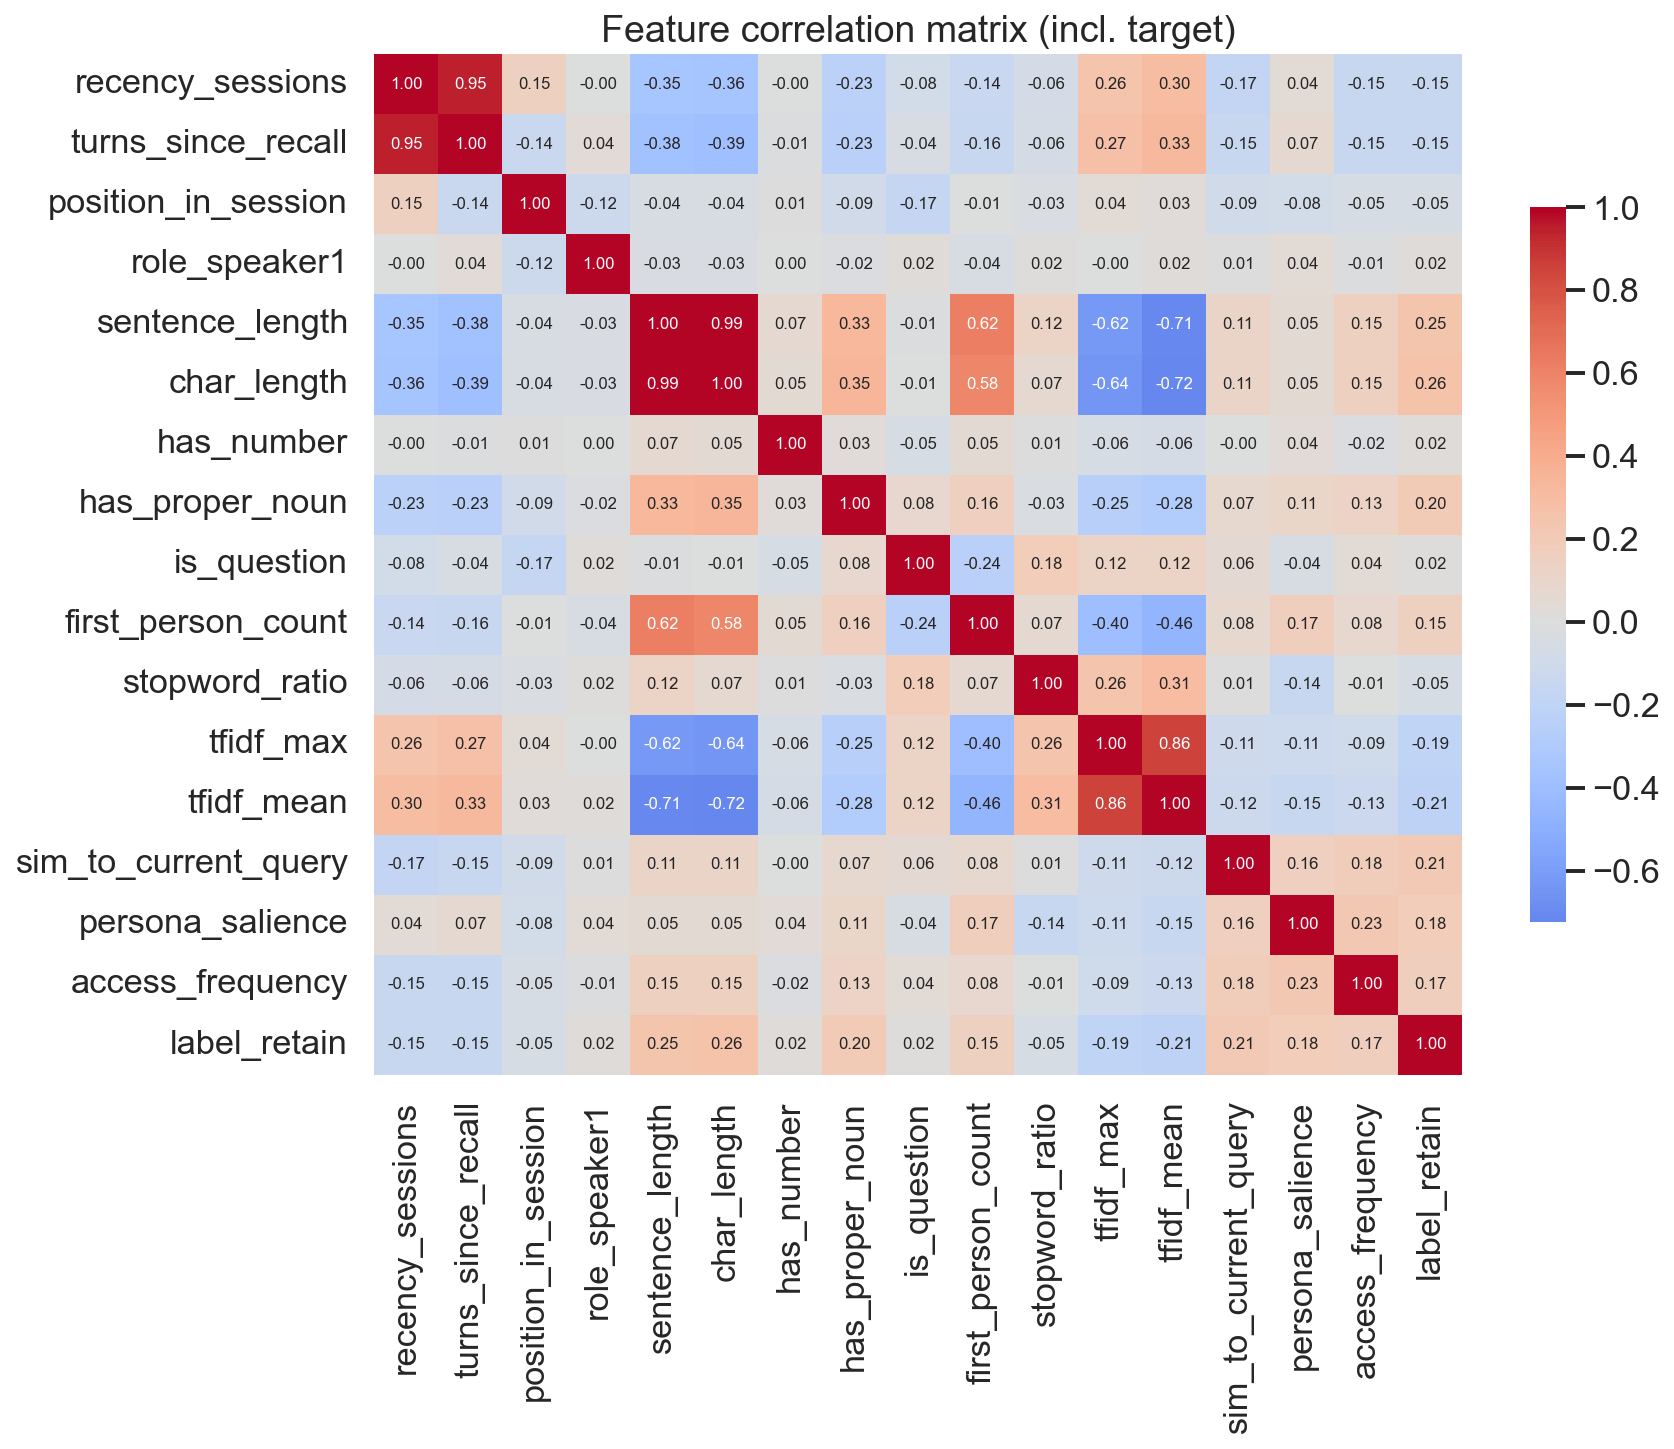
\includegraphics[width=0.52\textwidth]{correlation_heatmap.png}
\caption{Feature correlation matrix (including the target). Expected clusters
appear (length pair; TF-IDF pair) but no feature is collinear with the target.}
\label{fig:corr}
\end{figure}

\section{Reproducibility}
Public repository: \url{https://github.com/B-Raghav/Adaptive-Memory-Selection}.
Setup: \texttt{pip install -r requirements.txt};
install Ollama and pull \texttt{llama3.1:8b} and \texttt{dolphin-mistral}. Run, in
order, \texttt{src/download\_data.py}, \texttt{parse\_msc.py}, \texttt{features.py},
\texttt{labeling.py}, \texttt{train.py}, \texttt{evaluate.py},
\texttt{llm\_integration.py}; launch the demo with
\texttt{streamlit run app/streamlit\_app.py}. Notebooks 01--04 reproduce every
figure and table. Random seed $42$ throughout.

\section*{Statement of Contributions}
\small
Both authors jointly designed the study and problem formulation. R.~Beri led data
parsing, label induction and validation, feature engineering, and the LLM
integration and Streamlit demo. H.~Prakash led the modeling pipeline
(cross-validation, SMOTE, model comparison), evaluation figures, and the
experimental analysis. Both authors contributed to the report and presentation.

\end{document}
